\chapter{2DES im Magnetfeld}
\section{Zwei"=Komponenten"=Modell für ein 2DES auf dünnen Heliumfilmen}
\label{sec:theo_zweikomponenten}

\subsection{Motivation}

Messungen der Zyklotronresonanz eines 2DES auf dünnen Heliumfilmen (\cite{guenzler, Mis98}, siehe auch Abbildung~\ref{fig:guenzler_cr_abs}) zeigen eine Asymmetrie der Resonanzlinie, die bisher noch nicht zufriedenstellend erklärt werden konnte. Weiterhin wurde festgestellt, dass die Stärke dieser Asymmetrie von der Dicke des gesättigten Heliumfilms auf dem Substrat sowie von der Beschaffenheit der Oberfläche der verwendeten Substrate abhängig ist.

\begin{figure}[h!tbp]
	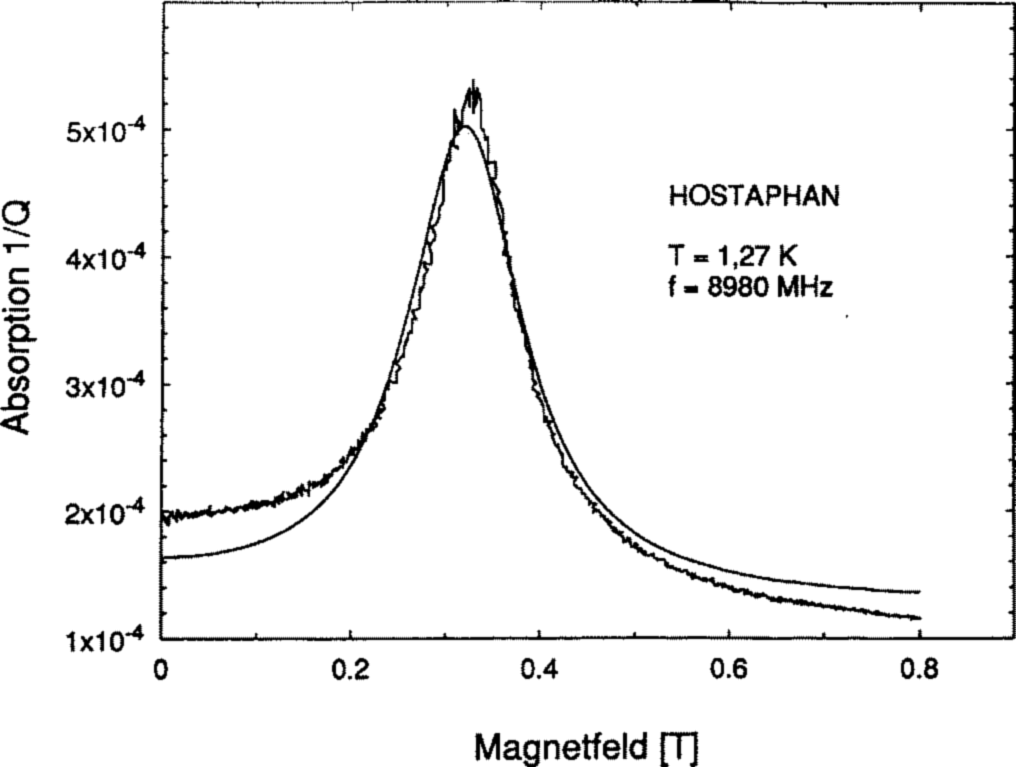
\includegraphics[width=\smidwidth]{theo_zweikomponenten/guenzler_cr_abs}%
	\hfill%
	\begin{minipage}[b]{\textwidth-\smidwidth-\tabcolsep}
		\caption[Zyklotronresonanzmessung aus \cite{guenzler}]{Messung der Zyklotronresonanz aus \cite{guenzler} an einem 2DES auf einer mit gesättigten Heliumfilm bedeckten Hostaphanoberfläche. Im hier gezeigten Absorptionssignal sieht man deutlich die starke Asymmetrie. Die gemessenen Daten können mit der herkömmlichen Kurvenanpassung (durchgezogene Linie) für die Absorption des Elektronensystems im externen Magnetfeld, basierend auf dem Realteil der Bewegungsgleichung für freie Elektronen \eqref{eqn:of_motion_real} nicht beschrieben werden.}
	\label{fig:guenzler_cr_abs}
	\end{minipage}
\end{figure}

Bisher wurde für die Absorption eines 2DES in Anwesenheit eines Magnetfelds der Realteil \eqref{eqn:of_motion_real} der aus der Drude"=Theorie erhaltenen Bewegungsgleichung für 2D Elektronen zur Anpassung der Messdaten verwendet.

Hierbei ist $\omega$ die Kreisfrequenz des elektrischen Feldes und $\omega_c=e\,B/m_e$ die Zyklotronfrequenz, die proportional zum äußeren Magnetfeld ist.
Der Imaginärteil der Bewegungsgleichung \eqref{eqn:of_motion_imag} beschreibt die Suszeptibilität des Elektronensystems, die direkt durch die Frequenzverschiebung der Resonatormode detektiert wird.

Bisherige Erklärungen für den Effekt der verstärkten Asymmetrie waren zum Beispiel eine Selbstlokalisierung der Elektronen bei Anwesenheit eines Magnetfeldes in einem Dimple, also die Erzeugung von so genannten Magnetopolaronen und auch die Oberflächenrauigkeit des Substrats wurde dafür verantwortlich gemacht.

Zusätzlich zu den Resultaten von \name{T. Günzler} \cite{guenzler} zeigen Messungen der Zyklotronresonanz auf PMMA"=beschichtetem Substrat von G.~Mistura \cite{mistura}, dass die beobachtete Asymmetrie mit abnehmender Filmdicke zunimmt. Daher liegt die Vermutung nah, dass die bei den hier verwendeten Substraten immer vorhandene Oberflächenrauigkeit für diesen Effekt eine entscheidende Rolle spielt. Das vorgestellte Zweikomponentenmodell versucht diese Beobachtung in eine Theorie umzusetzen, in der eine zusätzliche Komponente des Beitrages von an Substratrauigkeiten lokalisierten Elektronen berücksichtigt wird.

Die Grundidee des Modells ist zusätzlich zur Dichte freier Elektronen $n_e$ die Dichte lokalisierter Elektronen $n_l$ in die Berechnungen mit aufzunehmen. $n_e$ ist hierbei der Anteil, der bisher ausschließlich bei der Beschreibung der physikalischen Eigenschaften des Systems berücksichtigt wurde. Die Dichte $n_l$ bezeichnet den Anteil von Elektronen, der an Rauigkeitsspitzen des Substrats lokalisiert ist. Elektronen in dieser Klasse besitzen aufgrund ihrer lokalisierten Situation einen anderen Beitrag zum physikalischen Verhalten des Gesamtsystems. Für die gesamte Elektronendichte $n_s$ gilt also
    \begin{equation}
            \label{eqn:two_fraction}
            n_s=n_e+n_l\quad.
    \end{equation}

\subsection{Bestimmung des Anteils lokalisierter Elektronen}

Um die Größe der Dichte $n_l$ zu bestimmen, ist es nötig die Rauigkeit einer realen Substratoberfläche mit einfachen Parametern zu modellieren, so dass diese auch mit der Beschaffenheit der Oberfläche im Experiment vergleichbar ist. Im Folgenden soll auf die Grundlagen und vereinfachenden Annahmen des Zwei"=Komponenten"=Modells eingegangen werden. Bei der theoretischen Behandlung von 2DES im externen Magnetfeld in Abschnitt~\ref{ssec:2KM_anwendung} wird dann eine Anwendung des Modells auf die Erklärung des Verhaltens bei den Messungen der Zyklotronresonanz gezeigt.

\subsection{Modellierung des Heliumfilms}
Im Folgenden wird gezeigt, wie die Modellierung der Substratoberfläche nach \name{Klier} \ea{} \cite{Kli01,Kli02} durchgeführt wird.

\begin{figure}[h!tbp]
	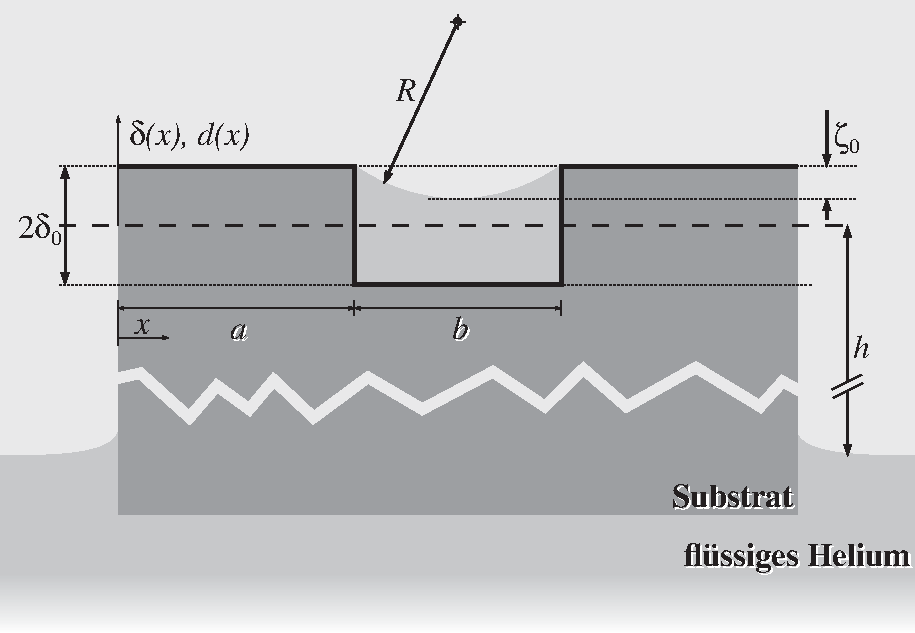
\includegraphics[width=0.5\textwidth]{theo_zweikomponenten/simple_surface}%
	\hfill%
	\begin{minipage}[b]{0.5\textwidth-\tabcolsep}
		\caption[Schema zur Berechnung des Verlaufs der Oberfläche des Heliumfilms]{Schema zur Berechnung des Oberflächenverlaufs $d(x)$ eines Heliumfilms bei bekanntem Substratverlauf $\delta(x)$. $R$ ist der Laplace"=Radius $R$ und $2\delta_0$ entspricht der Amplitude der Korrugation der Oberfläche.}
		\label{fig:simple_surface}
	\end{minipage}
\end{figure}
Zur Modellierung des Heliumfilms soll der Fall betrachtet werden, in dem die typische Längenskala der Oberflächenrauigkeit kleiner ist als die Kapillarlänge $\lambda$ des Heliums
	\begin{equation}
		\lambda=\frac{\sigma_\text{lv}}{\rho_\text{He} g}
	\end{equation}
mit der Oberflächenspannung des flüssigen Heliums $\sigma_\text{lv}$. Dies trifft zu für optisch glatte Substrate, wie sie für Messungen von 2DES auf Heliumfilmen üblicherweise verwendet werden. Für ein bestimmtes Oberflächenprofil $\delta(x)$ des Substrats kann man den Verlauf der Heliumoberfläche $d(x)$ mittels folgender Differentialgleichung berechnen:
	\begin{equation}
		\sigma_\text{lv}\frac{d''(x)}{[~1+(d'(x))^2~]^{3/2}} - \rho_\text{He} g
	        \delta(x) + \frac{\DC}{d^3(x)} = \rho_\text{He} g h\quad.
	\end{equation}
Für die vereinfachte Substratoberfläche aus Abbildung~\ref{fig:simple_surface} ergibt sich für $d(x)$ die Lösung
	\begin{equation}
		d(x)=
		\begin{cases}
			d_\text{top}=\sqrt[3]{\frac{\DC}{\rho_\text{He} g(h+\delta_0)}}&x<a\vee x>a+b\\
			2\delta_0-\zeta_0+R-\sqrt{R^2-(x-(a+\frac{b}2))^2}&a<x<(a+b)\\
		\end{cases}
	\end{equation}
	\begin{equation}
		\zeta_0=R-\sqrt{R^2-b^2/4}\quad.
	\end{equation}

\subsection{Modellierung der Substratrauigkeit}

Die Oberfläche der verwendeten Substrate ist optisch glatt. Ihre Rauigkeit bewegt sich in der Größenordnung von \unit[10]{nm} und kleiner. Falls nun ein Heliumfilm mit einer Dicke der gleichen Größenordnung auf dem Substrat adsorbiert wird, ist die Substratrauigkeit nicht mehr zu vernachlässigen. Hier soll eine raue Oberfläche, die als Grundlage für die weiteren Überlegungen dient, mit wenigen beschreibenden Parametern modelliert werden. Die Grundzüge der hier vorgestellten Rechnungen aus \cite{Kli02} stammen von \name{V. Tikhonov} \cite{Tik62}.

\begin{figure}[h!tbp]
	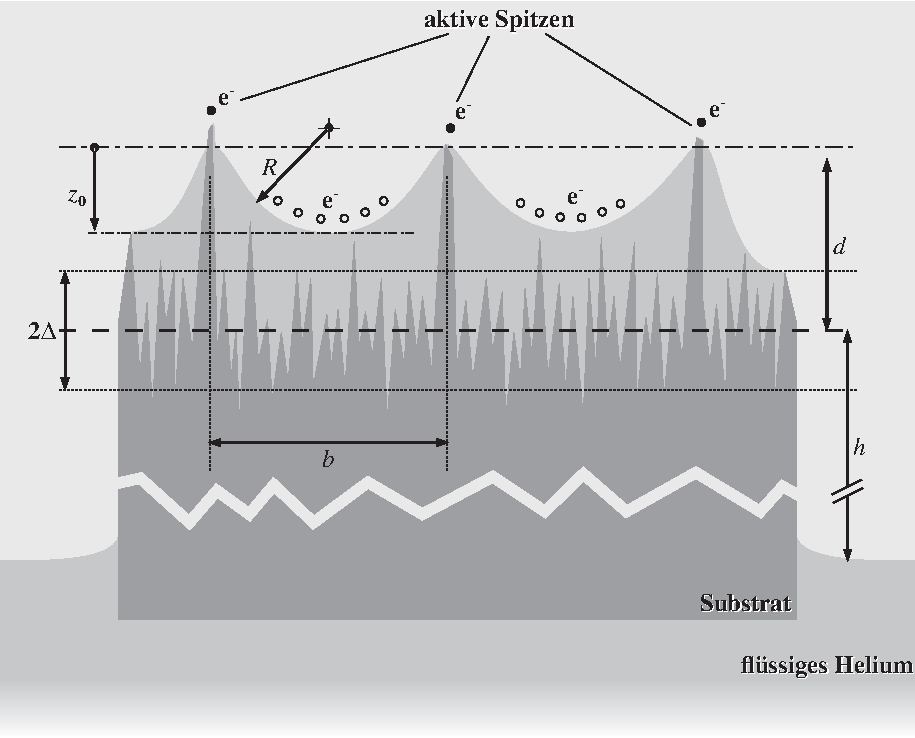
\includegraphics[width=0.7\textwidth]{theo_zweikomponenten/two-fraction_model}%
	\hfill%
	\begin{minipage}[b]{0.3\textwidth-\tabcolsep}
		\caption[Schematische Darstellung der Parameter der Oberflächenrauigkeit]{Schematisches Bild der Oberflächenrauigkeit und der hier verwendeten Parameter.}
		\label{fig:real_substrate}
	\end{minipage}
\end{figure}
Ein Substrat mit dem Oberflächenprofil $\delta(x)$ ist hier durch eine gaußförmige Amplitudenverteilung der Rauigkeitsspitzen charakterisiert
    \begin{equation}
        \label{eqn:Ddelta}
        G(\delta)=\frac1{\sqrt{2\pi\Delta^2}}e^{-\frac{\delta^2}{2\Delta^2}}\quad,
    \end{equation}
wobei $\Delta^2=\left<\delta^2\right>$ die mittlere quadratische Abweichung in vertikaler Richtung ist. Um die lateralen Eigenschaften der Oberfläche beschreiben zu können, braucht man auch eine Autokorrelationsfunktion für $\delta(x)$
    \begin{equation}
        \label{eqn:deltaAC}
        \left<\delta(x)\delta(x-x')\right>=\Delta^2 e^{-\frac{x'^2}{2\eta^2}}\quad,
    \end{equation}
hierbei ist $\eta$ die Korrelationslänge in horizontaler Richtung. Die Dichte der Spitzen oberhalb einer Höhe $\delta$, an denen Elektronen lokalisiert sein können, ergibt sich zu:
	\begin{equation}
		n_\delta=\frac1{2\pi \eta}e^{-\frac{\delta^2}{2\Delta^2}},
			\quad \eta=\left<\eta^2\right>\quad.
	\end{equation}
Um diese beliebige Höhe $\delta$ mit einem Laplace-Radius $R$ zu verbinden, nehmen wir an, dass für eine Laplace"=Länge $b$ im eindimensionalen Fall gilt:
	\begin{equation}
		b=n_\delta^{-1}\quad.
	\end{equation}
Wenn man Gleichung~\eqref{eqn:deltaAC} und die zweite Ableitung des Substratprofils $\delta^{\prime\prime}$ verwendet, kann man die Autokorrelationsfunktion folgendermaßen
    \begin{equation}
        \label{eqn:deltappAC}
        \left<\delta^{\prime\prime} \delta^{\prime\prime}\right> = \beta^2\equiv
        \frac{3\Delta^2}{\eta^4}
    \end{equation}
und die entsprechende Verteilung von $\delta^{\prime\prime}$ als
    \begin{equation}
        \label{eqn:Ddeltapp}
		D(\delta^{\prime\prime})= \frac1{\sqrt{2 \pi
		\beta^2}}e^{-\frac{{\delta^{\prime\prime}}^2}{2\beta^2}}	\end{equation}
schreiben.
Ein gesättigter Heliumfilm auf dem Substrat, dessen Profil mit $d(x)= d+\xi(x)$ definiert ist, wird das Substratprofil auf $\delta(x)$ abrunden. Infolge dieser teilweisen Abschirmung der Substratrauigkeit kann man, wie in Abbildung~\ref{fig:real_substrate} zu sehen, die \emph{aktiven Spitzen} (mit positiver Krümmung der Heliumoberfläche $d(x)$) und die \emph{passiven Spitzen} (mit negativer Krümmung des abschirmenden Heliumfilms) unterscheiden. Die Energie von Elektronen, die an aktiven Spitzen lokalisiert sind, ergibt sich folgendermaßen:
\begin{equation}
        \label{eqn:coupling_energy}
        V_a \ge -\Lambda/d_a,\quad \Lambda=\frac{e^2(\varepsilon_d-1)}{4(\varepsilon_d+1)},
        \quad \DC/d_a^3 \simeq \rho_\text{He} g h +\sigma_\text{lv}\sqrt{\left<\delta^{\prime\prime}
        \delta^{\prime\prime}\right>}\quad.
    \end{equation}
Hierbei ist $\epsilon_d$ die dielektrische Konstante des Substrats. Damit Gleichung~\eqref{eqn:coupling_energy} gilt, nehmen wir an, dass die lokale Ableitung $\xi''$ über den aktiven Spitzen kleiner ist als die korrespondierende Ableitung $\delta''$, so dass $\left<\xi''\xi''\right> \leq \left<\delta''\delta''\right>$ gilt.
    
Definition~\eqref{eqn:coupling_energy} zeigt, dass sich die Heliumfilmdicke an den aktiven Spitzen durch den vertikalen Abstand $h$ zur Bulk"=Oberfläche und einem zusätzlichen Laplacedruck zusammensetzt, der die Filmdicke reduziert.

Eine weitere wichtige Größe ist die Dichte der aktiven Spitzen $n_a$. Wir definieren:

	\begin{equation}
		\label{eqn:Dintegral}
		n_a^{-1/2}\int\limits_{\delta_c}^{+\infty}D(\delta) d\delta =
		(\zeta^2)^{1/2}~, \quad \zeta^2 \exp{(\delta_c^2/2\Delta^2)}\simeq
		n_c^{-1}
	\end{equation}
	\begin{equation}
		\label{eqn:screening_radius}
		n_c^{-1} +(R-\Delta)^2=R^2~, \quad
		\alpha/R \simeq \rho_\text{He} g h~, \quad  d\ll h\quad.
	\end{equation}

$\Delta$ ist in \eqref{eqn:Ddelta} und $\zeta$ in \eqref{eqn:deltaAC} definiert. Falls $h$ klein genug und deshalb $R$ verglichen mit $\Delta$ groß ist (z.\,B. $R^2\gg\Delta^2$), dann wird $n_c$ aus \eqref{eqn:screening_radius} vernachlässigbar, da $n_c^{-1}\simeq 2 R \Delta$ ist.
Unter diesen Bedingungen geht $\delta_c$ aus Gleichung~\eqref{eqn:Dintegral} gegen unendlich und die korrespondierende Dichte $n_a$ gegen Null. Wenn man die Höhe $h$ vergrößert, führt dies zu einer Verringerung von $\delta_c$, gleichzeitig wachsen $n_c$ und $n_a$.
Über die Bindungsenergie an den aktiven Spitzen kann man auch die Eigenfrequenzen $\omega_a$ der Lokalisierung einführen. Die Wechselwirkungsenergie ist von der Form
	\begin{equation}
		\label{eqn:VaDef}
		V_a\simeq-\frac{\Lambda}{d_a(x)}\ttextt{mit}
			d_a(x)\simeq d_r(0)\left(1+\frac{\delta''x^2}{2d_a(0)}\right)\quad.
	\end{equation}
Wenn man diese Energie um ihr Minimum an der aktiven Spitze herum entwickelt, erhält man
	\begin{equation}
		\label{eqn:VaExp}
		V_a(x)\simeq-\frac{\Lambda}{d_a(0)}+\frac{k_ax^2}2\ttextt{mit}
			k_a=\frac{\Lambda\delta''}{d_a(0)^2}\ttextt{und}
		\omega^2=\frac{k_a}m\quad.
	\end{equation}
Um die Gleichungen~\eqref{eqn:VaDef} und~\eqref{eqn:VaExp} zu erhalten, nehmen wir an, dass die Oberfläche des Heliumfilms in der Umgebung der Spitzen flach ist ($R^2\gg\Delta^2$) und somit der lokale Abstand $d(x)$ zwischen dem Elektron und der Position der Spitze allein abhängig von $\delta''$ ist.

